%%%%%%%%%%%%%%%%%%%%%%%%%%%%%%%%%%%%%
%                                   %
% Compile with XeLaTeX and biber    %
%                                   %
% Questions or comments:            %
%                                   %
% joshua dot mcneill at uga dot edu %
%                                   %
%%%%%%%%%%%%%%%%%%%%%%%%%%%%%%%%%%%%%

\documentclass{beamer}
  % Read in standard preamble (cosmetic stuff)
  %%%%%%%%%%%%%%%%%%%%%%%%%%%%%%%%%%%%%%%%%%%%%%%%%%%%%%%%%%%%%%%%
% This is a standard preamble used in for all slide documents. %
% It basically contains cosmetic settings.                     %
%                                                              %
% Joshua McNeill                                               %
% joshua dot mcneill at uga dot edu                            %
%%%%%%%%%%%%%%%%%%%%%%%%%%%%%%%%%%%%%%%%%%%%%%%%%%%%%%%%%%%%%%%%

% Beamer settings
% \usetheme{Berkeley}
\usetheme{CambridgeUS}
% \usecolortheme{dove}
% \usecolortheme{rose}
\usecolortheme{seagull}
\usefonttheme{professionalfonts}
\usefonttheme{serif}
\setbeamertemplate{bibliography item}{}

% Packages and settings
\usepackage{fontspec}
  \setmainfont{Charis SIL}
\usepackage{hyperref}
  \hypersetup{colorlinks=true,
              allcolors=blue}
\usepackage{graphicx}
  \graphicspath{{../../figures/}}
\usepackage[normalem]{ulem}
\usepackage{enumerate}

% Document information
\author{M. McNeill}
\title[FREN2001]{Français 2001}
\institute{\url{joshua.mcneill@uga.edu}}
\date{}

%% Custom commands
% Lexical items
\newcommand{\lexi}[1]{\textit{#1}}
% Gloss
\newcommand{\gloss}[1]{`#1'}
\newcommand{\tinygloss}[1]{{\tiny`#1'}}
% Orthographic representations
\newcommand{\orth}[1]{$\langle$#1$\rangle$}
% Utterances (pragmatics)
\newcommand{\uttr}[1]{`#1'}
% Sentences (pragmatics)
\newcommand{\sent}[1]{\textit{#1}}
% Base dir for definitions
\newcommand{\defs}{../definitions}


  % Packages and settings

  % Document information
  \subtitle[]{Le passé composé avec \lexi{être} et plus d'aliments}

\begin{document}
  % Read in the standard intro slides (title page and table of contents)
  \begin{frame}
    \titlepage
    \tiny{Office: % Basically a variable for office hours location
Gilbert 121\\
          Office hours: % Basically a variable for office hours
 lundi, mercredi, vendredi 10:10--11:10
}
  \end{frame}

  \begin{frame}{Annonces}
    \begin{itemize}
      \item L'atelier d'écriture vendredi
      \item[] \tinygloss{Writing workshop Friday}
    \end{itemize}
  \end{frame}

  \begin{frame}{La structure et les verbes}
    \begin{center}
      sujet $+$ \lexi{être} (conjugated) $+$ participle (with agreement)
    \end{center}
    \begin{itemize}
      \item DR and MRS VANDERTRAMPP
      \item[] OR...
      \item Verbs describing movement or a change of state
    \end{itemize}
  \end{frame}

  \begin{frame}{}
     \\
    \tinygloss{}
    \begin{columns}
      \column{0.5\textwidth}
        \begin{enumerate}
          \item
        \end{enumerate}
      \column{0.5\textwidth}
        \begin{minipage}[c][0.6\textheight]{\linewidth}
          \begin{center}
            \only<-3>{
              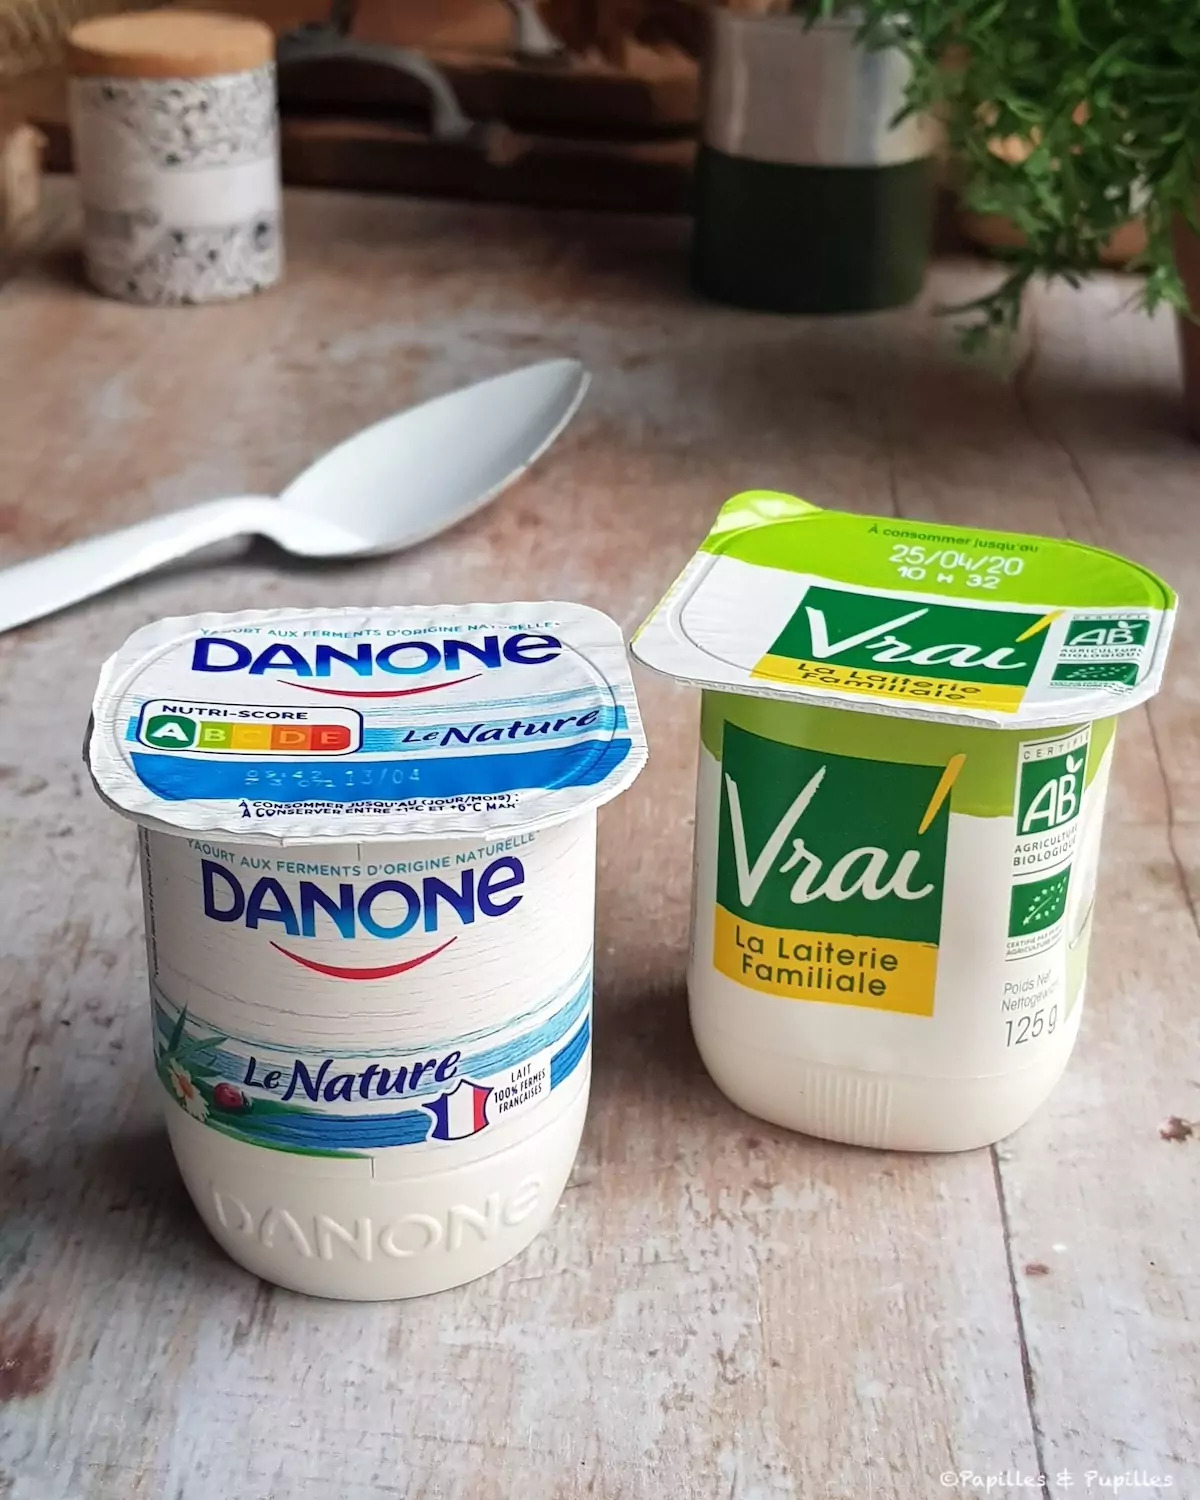
\includegraphics[scale=0.07]{yaourts.jpg}
            }
          \end{center}
        \end{minipage}
    \end{columns}
  \end{frame}

  \begin{frame}{}
    \begin{center}
      \Large Quiz
    \end{center}
  \end{frame}

  \begin{frame}{}
     \\
    \tinygloss{}
    \begin{description}
      \item[] \textbf{Modèle:} \emph{}
      \item[E1:]
    \end{description}
    \begin{columns}
      \column{0.5\textwidth}
        \begin{enumerate}
          \item
        \end{enumerate}
      \column{0.5\textwidth}
        \begin{enumerate}
          \setcounter{enumi}{}
          \item
        \end{enumerate}
    \end{columns}
  \end{frame}

  \begin{frame}{Mais pourquoi?}
     \\
    \tinygloss{}
    \begin{description}
      \item[] \textbf{Modèle:} \emph{}
      \item[E1:]
    \end{description}
    \begin{columns}[t]
      \column{0.5\textwidth}
        \begin{enumerate}
          \item
        \end{enumerate}
      \column{0.5\textwidth}
        \begin{enumerate}
          \setcounter{enumi}{}
          \item
        \end{enumerate}
    \end{columns}
  \end{frame}

  \begin{frame}{}
    \begin{center}
      \Large Questions?
    \end{center}
  \end{frame}
\end{document}
